\section{TEST RESULTS}

\subsection{Results Summary}

After completion of all testing, no IPCs dropped any messages during transit. This can be attributed to the ideal testing conditions. Hardwired network communication and single byte package size allowed for both TCP and UDP packets to be received despite UDP's lower inherenit reliability. The introduction of a wireless networks or lower quality routers may cause more of a differentiation to arise. The fastest overall system consisted of UDP network messages and ACH messages for the internal communication through the Pi. There was negligable difference in transit time between TCP and UDP over the network. Similar delays at this stage of the test can be attributed to the routers throughput. TCP response messages are processed at or below the microsecond accuracy level and does not impact our test results. A summary of all data collected is presented below for the network link in Table \ref{table:results summary net} and the internall Raspberry Pi link in Table \ref{table:results summary rpi}.

\begin{table}[h]
\caption{Results Summary: Network Link}
\label{table:results summary net}
\begin{center}
\begin{tabular}{c|c||c||c||c||c|}
\cline{2-6}
& \multicolumn{5}{c|}{Network: Link 1}\\
\hline
\multicolumn{1}{|c|}{Item} & UDP & TCP & ACH & ZMQ & ROS\\
\hline
\multicolumn{1}{|c|}{Average (ms)} & 3.834 & 3.829 & ZMQ & N/A & ROS\\
\hline
\multicolumn{1}{|c|}{Min (ms)} & 3.359 & 3.399 & ZMQ & N/A & ROS\\
\hline
\multicolumn{1}{|c|}{Max (ms)} & 95.063 & 42.006 & ZMQ & N/A & ROS\\
\hline
\multicolumn{1}{|c|}{Std Deviation (ms)} & 1.441 & 0.768 & ZMQ & N/A & ROS\\
\hline
\end{tabular}
\end{center}
\end{table}

\begin{table}[h]
\caption{Results Summary: Raspberry Pi Link}
\label{table:results summary rpi}
\begin{center}
\begin{tabular}{c|c||c||c||c||c|}
\cline{2-6}
& \multicolumn{5}{c|}{Raspberry Pi: Link 2}\\
\hline
\multicolumn{1}{|c|}{Item} & UDP & TCP & ZMQ & ACH  & ROS\\
\hline
\multicolumn{1}{|c|}{Average (ms)} & 3.834 & 4.774 & ZMQ & 3.752 & ROS\\
\hline
\multicolumn{1}{|c|}{Min (ms)} & 3.359 & 4.079 & ZMQ & 3.219 & ROS\\
\hline
\multicolumn{1}{|c|}{Max (ms)} & 95.063 & 43.974 & ZMQ & 73.533 & ROS\\
\hline
\multicolumn{1}{|c|}{Std Deviation (ms)} & 1.441 & 1.160 & ZMQ & 1.705 & ROS\\
\hline
\end{tabular}
\end{center} 
\end{table}

\subsection{UDP Results (Control)}

The control of this experiment utilized UDP messages over the network and UDP messages sent to the loopback address on the Pi. No missed messages occured despite UDP being the least reliable IPC method tested. Consistent results occured with a standard deviation of 1.441 ms and the average transit was 3.834 ms. This was the second fastest configuration tested. Figure \ref{UDP results} below shows a summary of collected data with outliers removed for clarity.

\begin{figure}[thpb]
 \centering
 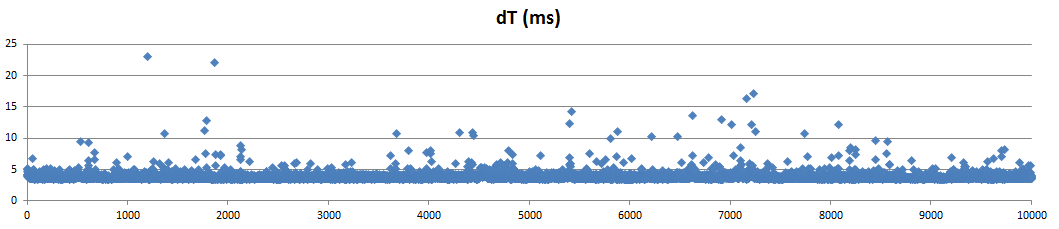
\includegraphics[width=1.0\columnwidth]{./images/udp2udp.png}
  \caption{UDP Control Test Results}  
  \label{fig:UDP results}
\end{figure} 

\subsection{TCP Results}

TCP was tested in both Link 1 and Link 2 configurations with UDP as the second link. No missed messages were recorded as expected for TCP. For the network link, TCP performed with negligable difference to UDP. This would suggest that for small data packets and reliable network connections the additional delay incurred by TCP's response message is negligable. Figure \ref{fig:TCP l1 results} below shows a summary of collected data with outliers removed for clarity.

\begin{figure}[thpb]
 \centering
 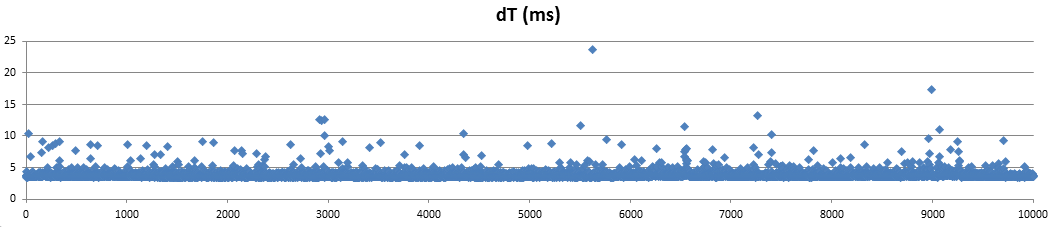
\includegraphics[width=1.0\columnwidth]{./images/tcp2udp.png}
  \caption{TCP Link 1 Test Results}  
  \label{fig:TCP L1 results}
\end{figure} 

Differentiation arises when TCP is utilized for the Link 2 loopback transport. Additional latency was recorded for an averate transit time of 4.774 ms and a standard deviation of  1.160 ms. This suggests the additional TCP overhead becomes an issue for embedded systems and would not be a valid candiate for an internal IPC. Table \ref{fig:TCP l2 results} below summarizes the Link 2 test results.

\begin{figure}[thpb]
 \centering
 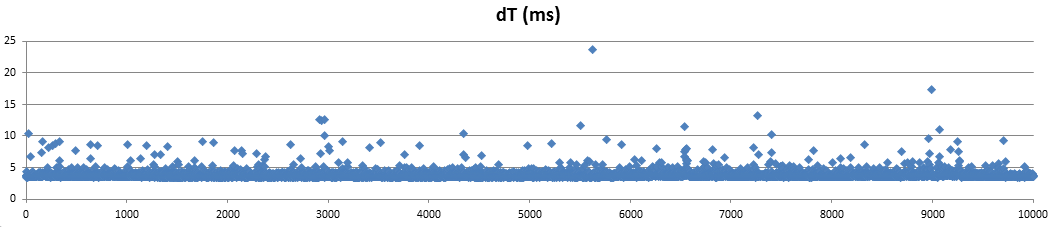
\includegraphics[width=1.0\columnwidth]{./images/tcp2udp.png}
  \caption{TCP Link 2 Test Results}  
  \label{fig:TCP L2 results}
\end{figure} 

\subsection{ZMQ Results}

placeholder for zmq results

\subsection{ACH Results}

ACH performed the fastest of all IPC methods tested. For consistency, UDP was used as the Link 1 transport over the ACHD library. ACHD can be configured as TCP or UDP messages and it was concluded that similar results would have been produced. Average transit time was 3.752 ms with a standard deviation of 1.705 ms. ACH exceeds the speed of UDP when transmitting internally and has the synchronization benefits of ZMQ without the additional latency observed. Figure \ref{fig:achresults} below shows a summary of collected data with outliers removed for clarity.

\begin{figure}[thpb]
 \centering
 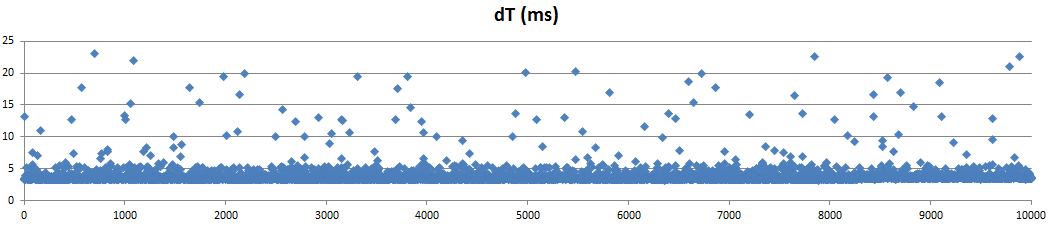
\includegraphics[width=1.0\columnwidth]{./images/achtest.png}
  \caption{ACH L2 Test Results}  
  \label{fig:achresults}
\end{figure} 

\subsection{ROS Results}

placeholder for ros results

